\chapter{Belle II Experiment}
\section{Belle II and SuperKEKB overview}
The fundamental goals of Belle II experiment are to search for evidence of New Physics in the luminosity frontier, and to improve the precision of the measurement of the SM parameters, such as $CP$ parameter.\cite{b2book} It uses SuperKEKB accelerator as its particle collider at the center-of-mass energy in the region of $\Upsilon(4S)$ resonances. The majority of the production will at the $\upsilon(4S)$ resonance that is slightly above the mass of two $B$ mesons. The electron and positron beams are designed at 7 GeV and 4 GeV, respectively, with boost factor of 0.28. This creates an environment for measuring time-dependent $CP$ violation by displacing the decay vertices of a $B$ meson pair in a measurable distance along the boosted direction. SuperKEKB has a targeted luminosity of $8\times 10^{35}\: \text{cm}^{-2} \text{s}^{-1}$, 40 times higher than its predecessor, KEKB at peak luminosity. The expected operation period is from 2019 to the end of 2030. These facilities are located in KEK, Tsukuba City, around 70 km in the north of Tokyo, Japan. Some key parameters of SuperKEKB are listed in Table \ref{tab:superkekb_pars}. The overview of SuperKEKB and Belle II are shown in Figure \ref{fig:superkekb_belle2}.

\begin{figure}
	\centering 
	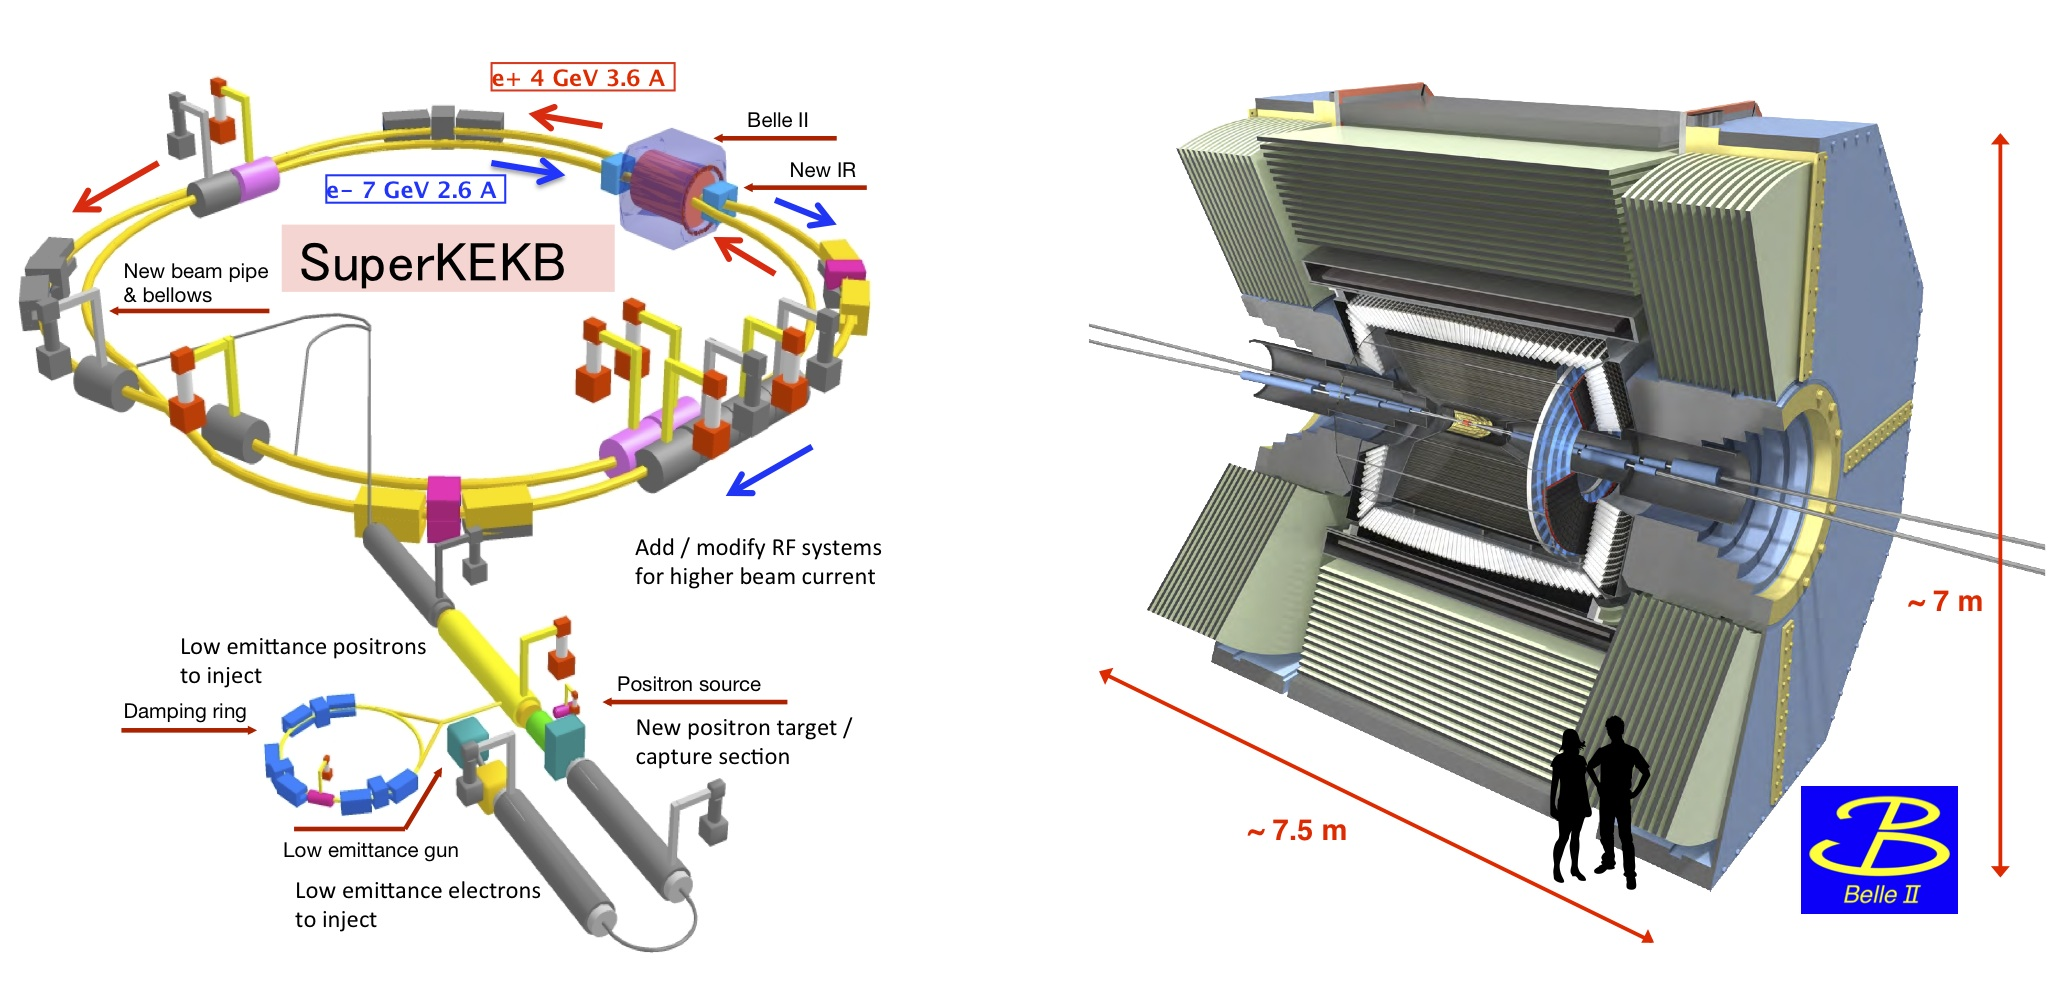
\includegraphics[height=7cm]{SuperKEKB-BelleII.jpg}
	\caption{Overview of SuperKEKB and Belle II detector \cite{Abe:2010gxa}.}
	\label{fig:superkekb_belle2}
\end{figure}

\begin{table}[H]
	\centering
	\large
	\caption{SuperKEKB parameters for low energy (LER) and high energy (HER) rings.\cite{b2book}}
	\label{tab:superkekb_pars}
	\begin{tabular}{c c c c}
		\toprule
		
		Parameters & LER($e^+$) & HER($e^-$) & Unit\\
		\hline
		Energy & 4.0 & 7.0 & GeV\\
		Half crossing angle & \multicolumn{2}{c}{41.5} & mrad\\
		Horizontal emittance & 3.2 & 4.6 & nm \\
		Emittance ratio & 0.27 & 0.25 & \%\\
		Beta functions at IP (x / y) & 32/0.27 & 25/0.30 & mm\\
		Beam currents & 3.6 & 2.6 &  A \\
		Beam–beam parameter & 0.0881 & 0.0807 & {}\\
		Luminosity & \multicolumn{2}{c}{$8\times 10^{35}$} &  $\text{cm}^{-2} \text{s}^{-1}$\\
		Perimeter of ring & \multicolumn{2}{c}{3} & km\\
		
		\bottomrule
	\end{tabular}
\end{table}


Belle II detector has a similar size as Belle so that it fits in the previous shell, but all sub-detectors and components have been either newly built or considerably upgraded. The advantage of SuperKEKB requires that Belle II has to be able to stably operate at 40 times higher events rates as well as 10 to 20 times higher beam background compared to Belle at its peak luminosity. This means the mitigation of the effects caused by such high beam background is essential to the success of Belle II. Higher background level leads to high occupancy and radiation damage to the detectors at close range, along with more fake hits in the vertex detectors, pile-up noises in electromagnetic calorimeter and neutron-induced hits in muon detector. Data-acquisition system (DAQ) and trigger are also upgraded not only to adapt to higher luminosity but also for low-multiplicity event sensitivity to support a broader search especially in dark sector. Belle II detector top view is shown in Figure \ref{fig:belle2_view}, and expected performances are summarized as follows: 


\textbullet \space vertex resolution of $B$ mesons of $\sim 50 \: \mu\text{m}$,

\textbullet \space excellent reconstruction efficiency for charged tracks down to several 100 MeV and fairly good efficiency for charged tracks down to $\sim$ 50 MeV,

\textbullet \space excellent momentum resolution up to 8 GeV/c,

\textbullet \space highly efficient particle identification to separate $\pi^{\pm}$, $\mu^{\pm}$, $e^{\pm}$, $K^{\pm}$ and $p$ at full energy range of experiment,

\textbullet \space full cover of experimental acceptance solid angle,

\textbullet \space ultra fast and highly efficiency DAQ and trigger system to cope with large data quantities and fast triggering frequency. 

\begin{figure}[htbp]
	\centering 
	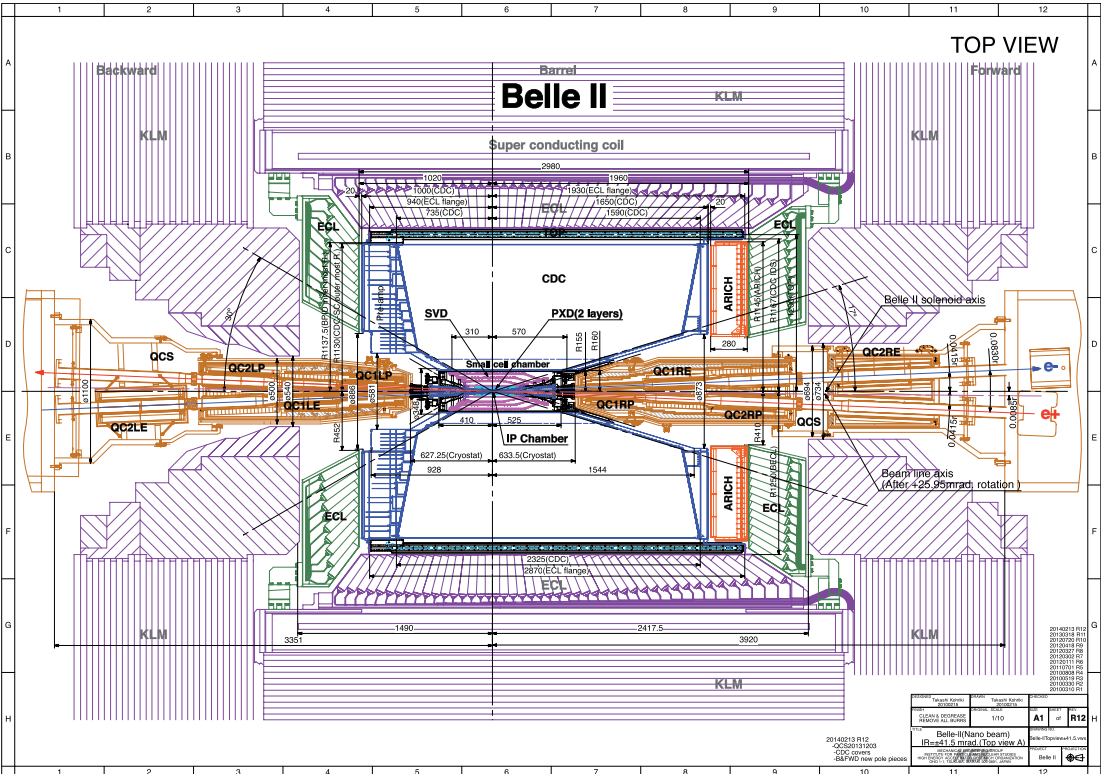
\includegraphics[height=10cm]{Belle2TopView.png}
	\caption{Belle II detector top view \cite{b2book}.}
	\label{fig:belle2_view}
\end{figure}

The success of Belle II detector depends on the complex of sub-detectors which each of them is design for specific purposes. The critical components and features are explained in the following sections. 

\section{Vertex detector (VXD)}
There are two components in VXD, the silicon based pixel detector (PXD) and silicon based vertex detector (SVD), where total 6 layers are placed in the inner-most region from interaction point (IP). As for PXD, two layers are placed at radii of $r=14$ mm and $r=22$ mm with DEPFET type pixel sensors, respectively. 
The PXD layers are the closest to Interaction point (IP) so the vertex resolution can be much improved. However, much higher events rate comes with much higher background level on PXD sensors. The overloaded occupancy leads to severe dead time and incredibly large data size from PXD if no data reduction scheme is implemented. In order to trim down data from PXD, a fast online tracking system is built up. In the data taking workflow, the data from PXD will be first readout to a system called ``ONSEN" which can store large size temporary data up to 5 seconds. In this timing window, a fast online tracking system will perform a track fitting extrapolate the fitted tracks backward to PXD plane so the region of interest (ROI) on PXD sensors can be defined. The data outside of the ROI are not read out from ONSEN system to external tapes where offline data is written. This scheme helps reduce large fraction of data especially in the very high luminosity.

For the SVD detector, the sensors are made of ``double-sided silicon strip sensors" (DSSD) with 4 layers at 39 mm, 80 mm, 104 mm, and 135 mm. The geometry of VXD from the is shown in Figure \ref{svd_geo}. The outmost layer of SVD is also larger than Belle SVD1/2. This could be helpful for ensure the reconstruction efficiency for the decay like $K_S^0 \to \pi^+ \pi^- $. However, the current hit filter of SVD doesn't allow the ``single-hit seeding" in the track recontruction, which means any track candidate should have at least two SVD hits. This is due to the concern of the large fraction of single-hit background. For the $K^0_S$ with long flight length, if the daughter $\pi^{\pm}$ only hits one layer of SVD, the reconstruction efficiency is dropped. 
\begin{figure}[H]
	\centering
	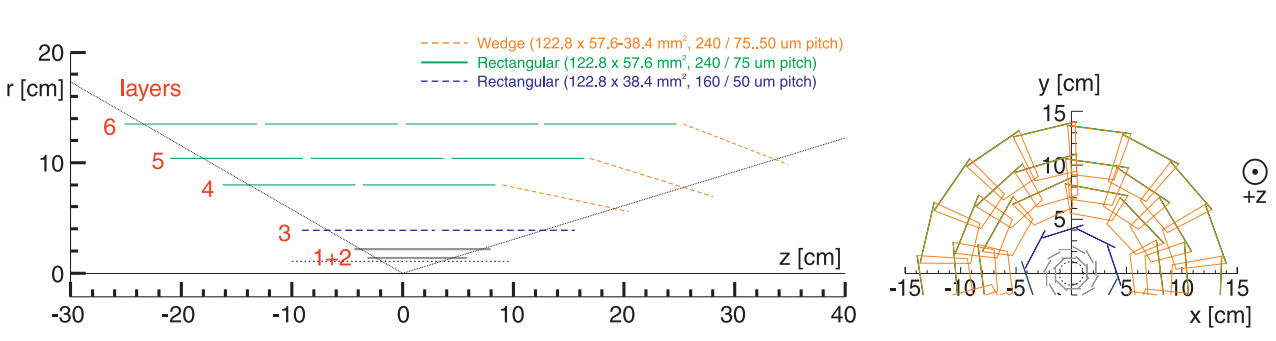
\includegraphics[height=4cm]{VXDGEO.png}
	\caption{A schematic view of PXD (2 layers in gray) and SVD (4 layers in green and orange) \cite{Abe:2010gxa}.}
	\label{svd_geo}
\end{figure}



\section{Central drift chamber (CDC)}
The central tracking system is the core component of spectrometer in Belle II, which consists of a fairly big drift chamber made of many small drift cells filled with He-C$_2$H$_6$ gas. The out radius of CDC has been extended to 1130 mm from 880 mm of Belle thanks to the much thinner layers in barrel region. The whole CDC contains 14336 sense wires in 56 layers, placed in the axial direction or the stereo direction. Such design can utilize the information from axial and stereo wires to construct a full 3 dimensional hits which forms helix tracks in CDC volume. Thus, CDC is one of the key components for measuring the helix parameters for tracking system. The example of CDC tracking of a cosmic ray event  is shown in Figure \ref{CDC_cosmic}

\begin{figure}[H]
	\centering
	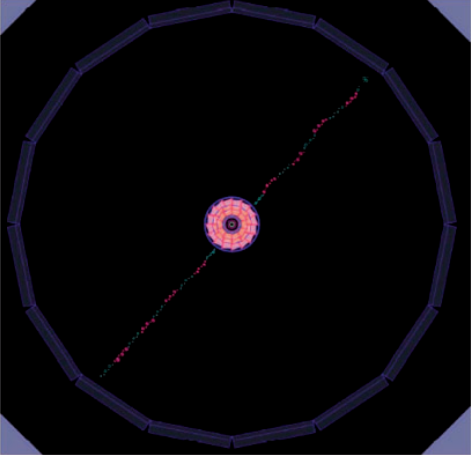
\includegraphics[height=6cm]{CDCcosmic}
	\caption{CDC tested with a cosmic ray event \cite{b2book}}
	\label{CDC_cosmic}
\end{figure}


\section{TOP and ARICH detectors}
The particle identification system of Belle II mainly consists of two parts, time-of-propagation counter (TOP) and aerogal based Cherenkov radiation imaging ring (ARICH). TOP is the specialized detector that can reconstruct Cherenkov radiation's time of arrival and generated position by a photon detector placed at the end of a 2.6 cm quartz bar. Due to the ultra-fast flying time of photon, the TOP detectors has to achieve timing resolution at around 100 ps. A 16 channels micro-channel plate photon-multiplier (MCP-PMT) with custom-made waveform electronics of readout is used. The resolution of starting time is achieved about 50 ps. \cite{Abe:2010gxa}. 

\begin{figure}[H]
	\centering
	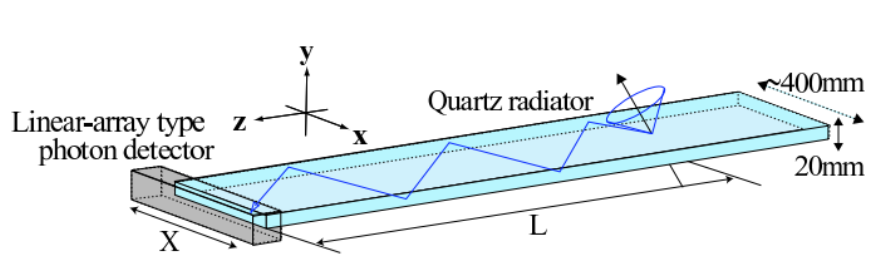
\includegraphics[width=0.7\linewidth]{top_mod}
	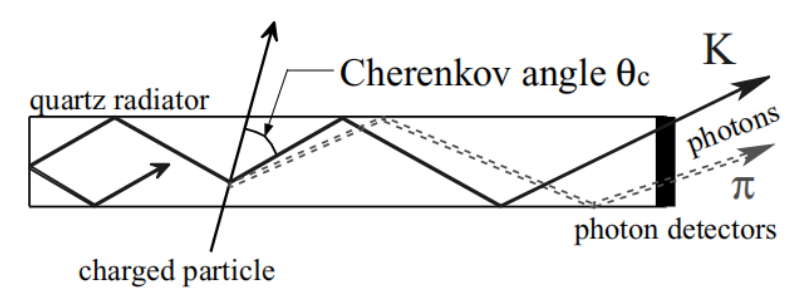
\includegraphics[width=0.7\linewidth]{top_img}
	\caption{Schematic view of TOP counter (up) and its imaging process of $K^{\pm}$ and $\pi^{\pm}$ (down)\cite{Abe:2010gxa}.}
\end{figure}

As for ARICH, it uses areogal as the sensitive material to approximately image the Cherenkov ring by a special focusing structure to identify charged particles. ARICH should be able to separate charged particles in a momentum range from 0.5 GeV to 4 GeV. ARICH requires single-photon-sensitive  high-granularity sensor to reconstruct the Cherenkov angle with small photon yield. Hamamatsu Corporation, Japan, has developed a hybrid avalanche photon detector (HAPD) to meet the requirements. Each sensor is $73 \times 73$ mm$^2$ embedded with 144 channels to accelerate emitted electrons in a 8 kV field. Avalanche photo-diodes (APD) are used for the detection of electrons at the end of electron acceleration, see Figure \ref{fig:arich_img}. The ARICH detector outlook and the ring image of cosmic $\mu$ on the HAPD sensors are shown in Figure \ref{fig:HAPD}.

\begin{figure}[H]
	\centering
	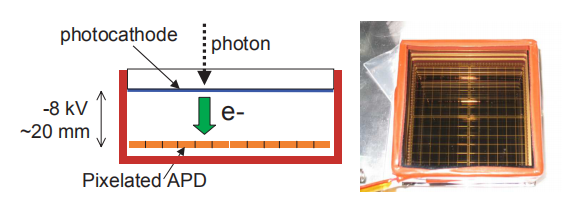
\includegraphics[height=5cm]{HAPD}
	\caption{Photon-electrons acceleration (left) and pixelated APD (right) at the end\cite{Abe:2010gxa}.}
	\label{fig:arich_img}
\end{figure}



\begin{figure}[H]
	\centering
	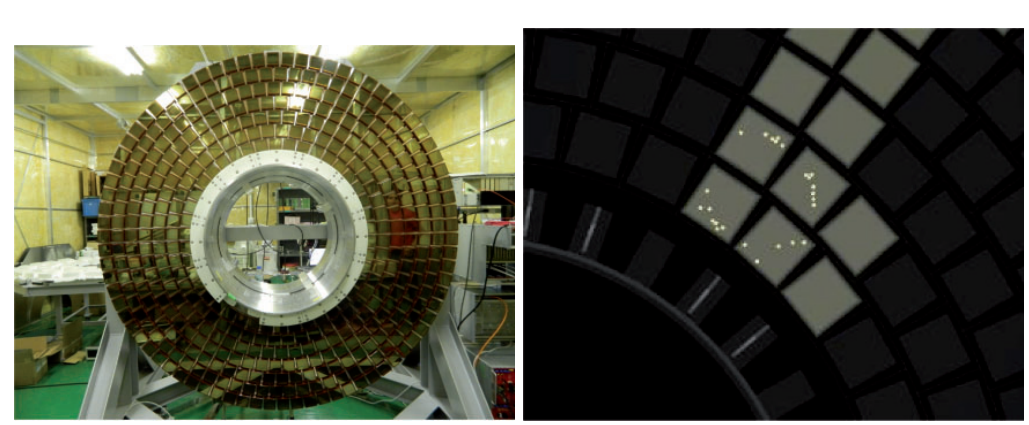
\includegraphics[height=6cm]{ARICH}
	\caption{ARICH detector (left) and the ring image of cosmic $\mu$ on the HAPD sensors\cite{b2book}}
	\label{fig:HAPD}
\end{figure}

\section{Electromagnetic calorimeter (ECL)}
The electromagnetic calorimeter of Belle II is mainly responsible for the detection of $\gamma$ radiation and electrons. The  thallium doped caesium iodide CsI(Tl) crystals are assembled tightly in all three different regions, backward/forward end-caps and barrel region. Compared to the previous ECL in Belle, the pre-amplifiers and the structures remain unchanged, while the readout  electronics have been upgraded. The estimated background level in Belle II ECL will cause the much longer decay time in the scintillation of CsI(TI). This will lead to the pile-up effect of readout noise. To compensate this effect, wave-form sampling electronics are embedded with the photon detectors (PMT). Especially in the forward direction of the electron beamline, where the level of beam background is much higher, the effect of pile-up noise becomes even worse and the performance of ECL will be of trouble if no special measure taken. In this situation, the pure CsI crystal is chosen as the material of detector to achieve a fast wave-shaping time and higher radiation tolerance compared to the dosed CsI(TI). 

\section{$K_L^0$ muon detector (KLM)}
KLM system of Belle II consists of a sandwich stacked iron plates and detectors at outside of the superconducting solenoid. The iron plates serve as the interaction materials with $>$ 3.9 times the interacting length of material compared to the ECL, allowing $K_L^0$ particles to shower through.
The Belle KLM material uses the glass-electrode resistivity plate chambers (RPC) which is not suitable for Belle II due to high background level.  Neutrons dose is significantly larger due to the much more electromagnetic radiation reaction on detector materials. The long dead time of RPC under such dose rate will reduce the efficiency of KLM. Besides, the mis-identification possibility would be raised so PID contribution from this part of detector will be meaningless. To mitigate this problem, the RPCs are replaced by the layers of scintillator strips with wavelength-shifting fibers, read out by silicon photomultipliers ( called ``SiPMs", Geiger mode operated APDs) as light sensors, which is proven to be able to reliably operate by setting up the discrimination threshold \cite{b2book}.

\begin{comment}
\begin{figure}[htbp]
\centering
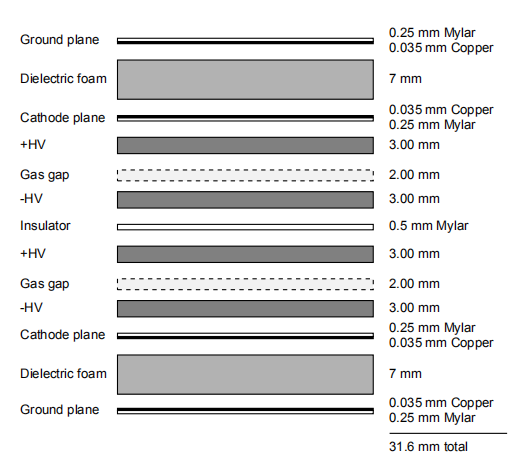
\includegraphics[height=10cm]{RPC}
\caption{ RPC layers structure\cite{b2book}}
\end{figure}
\end{comment}



\section{Trigger and DAQ system}
The interesting topics in Belle II physics analysis highly depend on the trigger system. With the upgraded capabilities to study a wide range of physics analysis at a very high luminosity in Belle II, the trigger system is expected to properly operate at a high event rate. The Belle II trigger system is composed of two levels: a hardware-based, low-level trigger called ``L1" trigger, and a software-based high-level trigger (HLT). The L1 trigger has a latency of $\sim 5 \mu\text{s}$ and the maximum trigger output rate is 30 kHz, which is limited by the read-in rate of data acquisition system (DAQ). Considered the high event rate and background level from future Belle II luminosity, a series of upgrades have been implemented for L1 trigger. The key improvements of L1 come from the firmware-based reconstruction algorithm and trigger logic. It's worth noting that a specialized set of hardware trigger lines for dark sector researches are implemented, which improves the trigger efficiency for single energetic photon in the final states. 

HLT, as the second level of Belle II trigger systema, plays an important role in DAQ. As discussed in the section of PXD, the data size in PXD is huge at high luminosity and the ROI selection must be applied to reduce the online event rate. The event rate reduction relies on the tracking extrapolation on PXD plane, which is the key function of HLT. HLT can suppress the event rate down to 15 kHz using the information from the CDC tracking and ECL reconstruction. The event rate is further reduced to 10kHz by using full reconstruction information. 

Since the primary goal of Belle II is focusing on $B$ physics studies, it is natural that the trigger system should be able to operate over all of the interesting $B$ physics conditions, with normally 3 or more CDC tracks and large energy deposition in ECL. By offline reconstructing the simulated events and studying the efficiency, close to 100\% $B$ decays are recorded by Belle II trigger system. However, the extensive capabilities of studying a large range of physics not only in $b$ sector brings a challenge to Belle II trigger and DAQ system. Belle II is expected to show the excellence at performing measurements on other important topics such as $\tau$ physics and dark sector researches. These topics usually suffer from the high beam background. Thus, the control of beam background becomes essential.
With SuperKEKB, beam background is about 10 to 20 times higher than Belle at the peak instantaneous luminosity. This rises a challenge for Belle II trigger and DAQ system. The main sources of beam background are beam-gas scattering, synchrotron radiation, the radioactive Bhabha scattering, the two-photon process, beam-beam effects, and Touschek effect. Their impacts depend on many factors such as beam current, luminosity and vacuum conditions, etc. One of the featured topology of these beam background events is the combination of two charged tracks in CDC and one or two clusters in ECL. Beam background events are often assembled with low-multiplicity events from primary collision, and the latter is the main focus of dark sector studies. It's quite important to distinguish these low-multiplicity events from various beam backgrounds. The simulated beam background rate and their sources are listed in Table \ref{tab:BG}.

\begin{table}[htbp]
	\centering
	\large
	\caption{Simulated beam background rate (12th BG campaign)\cite{b2book}}
	\label{tab:BG}
	\begin{tabular}{c c c}
		\toprule
		Type & Source & Rate (MHz)\\
		\hline
		Radiative Bhabha & HER &  1320\\
		Radiative Bhabha & LER &  1294\\
		Radiative Bhabha(wide angle) & HER &  40\\
		Radiative Bhabha (wide angle) & LER &  85\\
		Touschek scattering & HER &  31\\
		Touschek scattering & LER &  83\\
		Beam–gas interactions & HER &  1\\
		Beam–gas interactions & LER &  156\\
		Two-photon QED & - & 206\\
		\bottomrule
	\end{tabular}
\end{table}

The improvements on both L1 and HLT triggers, along with DAQ upgrade has shown a good potential in dark sector researches\cite{de2018first}\cite{macqueen2020dark}, thanks to the improved discriminating ability of low-multiplicity events against beam background. In future, several modifications on the current trigger system is under consideration, such as the partially pre-scaled trigger lines, which is expected to be optimized for dark sector studies\cite{b2book}. 


\begin{comment}
Based on the reasons discussed above, Belle II trigger has been designed to have 2 separated levels of triggers. Low level trigger, also called as L1 trigger, is hardware-based trigger. and high level trigger (HLT) is the software based trigger.
The L1 trigger rate can go up to 30kHz that is also the up-limit of DAQ read-in rate. The latency of L1 is control to be 5 $\mu$s, improved from Belle trigger.
And yet 30kHz is still to high for writing out the data to tape, so the HLT must be implemented to reduce the trigger rate to about 10kHz and it has to be able to select ROI on the PXD to reduce the data flux limited by bandwidth of read-out cables. To do that, HLT utilize  the full offline reconstruction algorithms to allow the access of full-granularity
event reconstruction using all detectors except for the PXD. 

\end{comment}

%2021.01.27 ends here
\begin{comment}
\section{Detector simulation}
The Belle II simulation makes a use of GEANT4 software. GEANT4 package can accept the event created by module called ``particle gun" which directly injects particles to detector volume. Or it takes in software simulated data, which in general is called ``event generator". Belle II Analysis Framework (BASF2) software (see the next section for the details of BASF2) provides the interface for createing simulated data from event generator to GEANT4. Most of the primary particles are simulated by event generator and sent to GEANT4 for simulation between detectors' components. The out-flying particles that has relatively long life time compared to the primary interaction such as $K_S^0 \to \pi^+ \pi^-$ are simulated in GEANT4 after the event generator does its job. Exchanged bosons and primary electrons(positrons) will not be feed into GEANT4. Then GEANT4 creates secondary particles during the particle interaction and detector material, such as the radiations from charged tracks and also the scattering processes with detector materials. The hits digitization are generated by other BASF2 modules using primary and secondary particles together. Finally, the response from detectors are sent to the persistent data storage (called ``DataStore" as C++ objects, detail in next section.) to be used in the analysis chain of BASF2. 

For each type of the particles and each type of detector material, the interaction is varied in different processes. The co-responding process of physics should be specified by the users or using the provided list from GEANT4 developer group. In Belle II simulation, the
Fritiof quark–gluon string model at high energy and the Bertini intra-nuclear cascade model at low
energy are used by default from GEANT4 list. 

The simulation of the beam background is done by a software called SAD, as external part of BASF2. It simulates the flux of particles from the beamline of the SuperKEKB accelerator. Whenever a particle trajectory deviates from the beamline region and hit the Belle II detector part, its momentum and position vectors will be saved into a configuration file. Then such configuration file will provide the initial information for GEANT4 simulation software to simulate the interaction between the given particle and Belle II detector, which is eventually analyzed as normal particles by BASF2.
The output of BASF2 is standard ROOT format and it presents how a beam induced particle interacts with detector material to create simulated hits as beam backgrounds. 

The mixing of background is then implemented to provide a realistic view of physical events and beam background overlay. Since the format of beam background is simulated hits, thus adding the background events is done by injecting the simulated hits, then move to the digitization of hits to detector responses. In a event time window $\Delta t$, assuming the given type background has a average rate of $R$, the mixing number of background hits in such event is: 

\begin{equation}
\bar{N} = sR\Delta{t}
\end{equation}

$s$ is optional scaling factor which can be used to study the influence of given type background in different level. Because $R$ is averaged value, in the actual mixing, the number of $\bar{N}$ is used as the expected value of Poisson distribution, which presents the number of observed events when many trials of such events is made with certain small possibility per event.  In order to simulate the effect of timing different of background and physical events, the mixing timing window over $\Delta t$ is randomly shift according to the physical events.
With the real experimental data comes in handy, the method of adding background events to physics events is slightly different since using real beam background can provide a more precise result than simulation. By setting a random trigger for beam background, the hits digitization from real beam background will be collected and add to simulated physics events. Although the pile-up noise collected in this method is not very precise because of the threshold set for detectors allowing only part of noise to be added, the non-recorded noise can still contribute to the pile-up noise for physics events, and they are not included in this method. Yet overall it provides a more realistic evaluation of beam background overlay.

\end{comment}

\section{Analysis Software} 
The data acquired by the Belle II experiment or simulation can be processed by  Belle II Analysis Software Framework, called BASF2. It has a good capability to handle the tasks of sophisticated algorithms for simulation, reconstruction, visualization, and analysis. The official BASF2 is developed in different release versions, light-versions and featured-versions. In this thesis, release-05-01-01 version is used. 

\subsection{BASF2 Core Structure}
The core structure of BASF2 contains three major parts: the analysis codes specifically required by the needs of Belle II data (called Belle II codes), the external libraries that are the third-party software which Belle II utilize, and the tools for configuring and installing the BASF2 software. 

The Belle II codes consists of many packages. They are categorized based on the different levels of Belle II detector components, like the packages of base-level system control called ``framework", the package for track reconstruction called ``tracking", and the one for post-reconstruction data analysis called ``analysis".
Users can work either with compiled binary version of BASF2 installed centrally on working servers, or build from the source based on their own need. 

As for the externals, it contains the many packages or libraries that provide functionalities BASF2 needs during the execution or installation. For example, some basic packages, like gcc compiler, cmake, tar, wget, Python and git are included. In particular, due to the dependence of the analysis tools that may be frequently used by Python, around 100 additional Python packages are installed as the externals, such as ``Numpy" and ``matplotlib" packages that provide functions for statistical calculations and plotting. The complexity of building all of these external software could be tough for users so that the compiled versions that cover the common platforms are available from BASF2 official repository. 

Tools are collections of shell or Python scripts for setting up BASF2 and externals environment. It can easily handle the need of setting up an environment of specific BASF2 version and the externals tied to that version. It also provides a function to setting up the environment of developing BASF2, where developers can get one developing copy of BASF2 and write the additional codes as the modification, so the compatibility of BASF2 could be easily maintained by building a release version from the developing branches. In this thesis, two new packages are developed and built with release-05-01-01 version BASF2. This developing version of BASF2 contains all functions that release-05-01-01 has. The details will be discussed later. 

\subsection{Event Processing Workflow}
The data from Belle II detector or from the simulation, are organized into a set of runs that are defined by either experimental conditions or simulation conditions. For instance, the simulation data from a certain detectors' condition are packed together, marked with the conditions' database index that is used during the simulation.  Such data sample then is divided into different runs based on estimated luminosity from experiment, which can contain the different number of events in each run.  This scheme is used for categorizing experimental data as well, so that users can easily know which experiment conditions are used. 
 In a run, every event is recorded as an independent measurement of  an electron-positron collision, a cosmic ray injection or background event. Such experiment-run-event structure is the basic data structure that BASF2 handles. Thus, when BASF2 processes a data set, the functions are called for every event based on different configurations that are corresponding to the different experiment conditions. For example, in a data set where events are recorded with the different magnetic fields, BASF2 can automatically change the configurations of the magnetic fields event-by-event to provide a better track measurement. Based on this idea, all BASF2 functions (called ``modules") are developed based on a python module class which contains following embedded functions to be called at event-based level: 


\textbullet \space initialize: called at the start of processing a event to properly set up constants needed for this run.

\textbullet \space beginRun: called at the start of calling this module, including setting up database conditions used in this run (run-dependent configurations) or event (event-based configurations).

\textbullet \space event: called for each event. This is the actual processing step, such as perform tracking or combining all daughters to find a mother particle. 

\textbullet \space endRun: called at the end of a run, usually to register all processed information to the storage, such as physics variables from all reconstructed particles.

\textbullet \space terminate: called at the end of the processing of all events, release the buffered space and memory.

BASF2 executes a series of modules loaded dynamically to process the data set according to above sequence. The selection, configuration and executed order of the modules are defined by a file called ``steering file" written in Python. The modules parameters are attributes which can be set during the runtime using the steering file. For example, the ``Path" object declared in a steering file stores the sequence of modules that will be executed, to which allow other modules such as ``mdstInput" or ``reconstructDecay" to be added.
Users can use ``boolean" type variable set in ``event" function to create a conditional branch of a ``Path" in case that one event needs to be processed with different modules at the same time. For instance, in the decay reconstruction package, if a decay chain is not fulfilled by missing one particle in the ``event" functions, other back-up decay chains can be checked to see if a successful reconstruction is possible.  

The object that interacts with BASF2 I/O is called ``DataStore". This implementation doesn't depend on the event data model. The only mandatory component is called ``EventMetaData" which presents the experiment, run  and event number of a event. ``Unpacker" module converts the raw digits into digits-based object in BASF2. In simulation, digitization is done by module called ``digitizer". The digits-based objects are further processed to form hits or clusters depending on detector types. Higher level functions such as tracking and decay reconstructions are implemented based on these basic information by their packages. Eventually, BASF2 writes out the information based on users' needs, like kinematics variables, to ROOT\cite{ROOTcern} format files, or simply prints out processing statistics to the standard output.

 In practice, BASF2 starts running when it checks there is at least one module specifying the number of events to be processed in a ``path"  from the ``steering file", then it reads in the information from ``DataStore" in the input ROOT file, execute all the requested modules in the ``steering file" and return the time and number of events as information printed in standard output. In Figure  \ref{fig:basf2_eg}, an example of ``steering file" is shown, with a ``path" called ``main" created and a module called ``EventInfoSetter" added. This steering file will process 100 event, set their experimental numbers, run numbers and event numbers.

\begin{figure}[htbp]
	\centering
	\includegraphics[height=6cm]{BASF2-steering}
	\caption{ An minimal example of BASF2 steering file, setting up a basic processing of 100 events in ``path" called ``main". }
	\label{fig:basf2_eg}
\end{figure}





\subsection{mDST structure}

The output from BASF2 processing can contain several detector-specific objects, which are restored as mini data summary table (mDST) type ROOT file. For instance, in a mDST file, the object called ``RecoTracks" will be created if track pattern recognition is called and ``Track" object will be created if the track fit is performed. For a mDST level analysis, the goal is usually aimed to find particles from physics processes and reconstruct decay information. A output mDST ROOT file could typically contain the following objects:

\textbullet \space Track: object presenting any charged particle trajectory. It's linked to multiple track fit results using different nominal mass hypotheses as well as their track fit quality to help select good tracks.  

\textbullet \space TrackFitResult: the fitting result of tracks with different mass hypotheses. It consists of five helix parameters, their covariance matrix and p-value from the fit. It also stores the information of hit pattern on vertex detector and CDC. 

\textbullet \space V0: object for the relative long-lived neutral particles that fly out of interaction region but mostly decay or interact inside detector region. In Belle II, these are mostly $K_S^0$, $\Lambda$ and photon converted to electron pairs. V0 also stores their relation to the charged daughter tracks and track fit results for further selections.


\textbullet \space PIDLikelihood: it presents for the possiblity of a charged track to be an electron, muon, charged kaon and pion, proton and deuteron provided by particle identification system. 

\textbullet \space ECLCluster: reconstructed cluster in ECL detector. It consists of energy deposition and hit positions as well as other hit shape related variables. If a cluster is matched with an extrapolated track, a relation between them will also be created. 

\textbullet \space Reconstructed cluster KLM detector. It consists of momentum and position measurement. If a cluster is matched with an extrapolated track, a relation between them will also be created. 

\textbullet \space KLId: $K_L^0$ candidates with the particle identification as related to KLM and ECL clusters. 

\textbullet \space TRGSummary: L1 trigger information. 
 
\textbullet \space SoftwareTriggerResult: HLT information mapped by trigger names to trigger results. 

\textbullet \space  MCParticle: simulated particles containing 
momentum, production and decay vertex, relations
to mother and daughter particles, and traversed detector components. Particle-detectors relations are
created if simulated particles are correctly reconstructed as
tracks or clusters.

The size of mDST level data is very important to BASF2 offline processing performance. Thus, mDST level data is restricted from contain non-physical analysis related information such as raw digits or calibration constants. For detailed detector
or reconstruction algorithm performance studies, and also for calibration tasks, a dedicated format higher than mDST, called cDST 
(calibration data summary table), is used.
 

%2020.01.28 ends
\subsection{Conditional Database}

In addition to the physics data, analysis relies on various conditional data that are different calibration of detector, weight files for multi-variate analysis usage like PID and so on. This data is stored in a central database server called central Conditional Database (CDB). 

Conditions are made of payloads and each payload has its own``Intervals of Validity" (IoV). It defines in which runs the payload is valid. A set of payloads and IoVs are called a global tag (GT). Considered the GT that is required by the different analysis purposes may change even though the experiment condition is still same, GT is subjected to be updated once new calibrations of detectors or weight files for MVA tools are available. On the users' side, except for just using central database, a local database back-end that takes GT information such as calibration data while uses a local database, such as a customized PID weight file,  is also possible.  It automatically download the needed database files that are required for a BASF2 execution and stores them in a local folder. This means even if the computer is offline or the CDB is not reachable, one can still run BASF2 as long as the local folder was there. 

\begin{figure}[htbp]
	\centering
	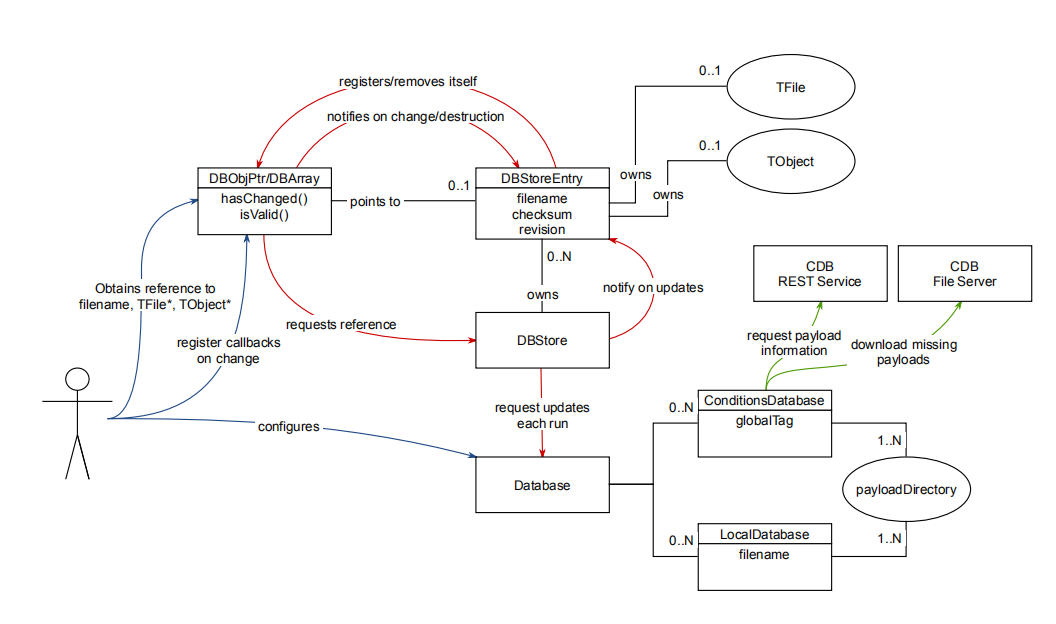
\includegraphics[height=9cm]{CDB}
	\caption{ Relations of all entities in CDB\cite{BASF2}, showing the management logic from users' end to each CDB files and services. }
	\label{fig:CDB}
\end{figure}

The management of CBD with the extension of local database gives a good convenience for users to perform their own analysis and share the results with collaborators.
Users' access to conditions objects in the CDB is
provided by two interface classes, one for single objects
called ``DBObjPtr" and one for arrays of objects called
``DBArray". To facilitate easy creation of new conditions data – for example, during calibration – we provide two payload creation classes, ``DBImportObj" and ``DBImportArray". They
have an interface very similar to DBObjPtr and DBArray\cite{BASF2}.
Users instantiate one of the creation classes, add objects
 to them and commit them to the configured database with a user-supplied IoV. This includes the support for run dependency as well. The capability to use a local file-based
 database allows for easy preparation and validation of
new payloads before they are uploaded to the CDB. The scheme of this entities and how users interact with CDB object is demonstrated in Figure \ref{fig:CDB}. For example, user can perform their analysis and first locally generate weight files or calibration data based on different run conditions and reconstruction criteria, which are stated by their names of the IoVs. Once the results are good to share, they can create a GT in CDB of which they have the full ownership, add all database files into the GT and open it to Belle II collaboration. Anyone who would like to re-calibrate data or use their weight files for PID and so on, can simply use the built-in function ``basf2.useCentralDB()" in BASF2 to directly access the corresponding data. However, only the creator of the CDB objects has the right to add, recall, replace and remove the GT, which guarantees the stability of the CDB and responsibilities for each user.


\begin{comment}
\subsection{Summary}
BASF2 has been developed for an emphasis on providing reliable and high quality performance for Belle II analysis. It satisfies the most of demanding requirements of data taking, simulation, reconstruction, and offline analysis. 
\end{comment}

\section{Belle II simulation}

This section briefly describes simulation (MC) used in the studies presented in this thesis. As for the focus of this analysis is in $b$ sector which is mainly from $\Upsilon$(4S) decay, the discussed simulation is based on the collisions with center-of-mass (CMS) energy at $\sqrt{s} = 10.58 $ GeV.

In the previous section, it's shown that many packages and functionalities have been integrated with BASF2, including the core components of Belle II simulation in $B$ decay: ``evtgen" as event generator and ``GEANT4" as the simulator of detectors. Along with the active development of BASF2 in the early stage of Belle II, the versions of software that is used for simulation and reconstruction are often different. For the simulation used in this analysis, BASF2 version release-04-02-08 was used. For the event reconstruction, the used BASF2 version is release-05-01-01. This is not a problem thanks to the CDB management, allowing modified software to use the same constants such as magnetic field distribution for the consistence between simulation and reconstruction.

 All simulations start with at least one event generator that configures the physics processes. In Belle II, the configuration of ``evtgen" requires a decay file called ``xxx.dec" that describes the decay chain from a certain mother particle, branching fraction for all processes and decay-related information such as flavor mixing or $\it{CP}$ violation information. For different type of decays, the different decay files are prepared. MC sample is centrally produced using Belle II GRID computing service based on these files periodically, so that the latest improvements of software can be applied. Each round of MC sample is called a campaign named with their index, such as ``MC13", which is the 13th (latest in 2020 Winter) Belle II official MC production (in the following content of this thesis, MC13 will be used referring this group of MC samples). 
 
 For the analysis in this thesis, there are two MC samples, one is called ``signal MC" and the other is called ``generic MC". Both MC samples use ``evtgen" as event generator. Signal MC, as its name suggests, is the MC sample that describes the whole decay chain of $B^0 \to K_S^0  K_S^0  K_S^0$. The mother particle of the decay chain is $\Upsilon$(4S), then it decays into a pair of $B^0-\bar{B}^0$ at branching fraction of 100\%, with the model ``EvtVSSMix"\cite{evtgen} describing the decay model. Then, one of the $B$ meson is set to decay into three $K_S^0$ based on phase-space model (``PHSP") at 100\% branching fraction. To be noted, the phase-space model doesn't provide any time-dependent $\it{CP}$ violation. The default configuration of ``evtgen" can not handle multi-bodies charmless $B$ decay with TDCPV. A modified decay model profile is under-development and not fully validated yet. Thus, MC sample of $B^0 \to K_S^0  K_S^0  K_S^0$ yields zero $\it{CP}$ parameters by default. As for the other $B$ meson, it decays into all possible final states that are described by Belle II generic decay file. 
 
 As for generic MC, all hadronic processes in a  $\sqrt{s} = 10.58 $ GeV collision are simulated. The total production cross section receives contributions from not only $\Upsilon$(4S) ($b$ -flavor decay dominated), but also $u, d, s, c$. 
 Their relative branching fractions are taken from cross sections at  $\sqrt{s} = 10.58 $ GeV as shown in Table \ref{tab:generic_br}. Generic MC sample contains 6 types of MC samples due to this production arrangement, where $\Upsilon$(4S) produces ``mixed" (neutral) and ``charged" $B$ meson pairs and the rest are ``uubar", ``ddbar", ``ccbar" and ``ssbar", respectively. In this thesis, the latter 4 types of MC samples are combined and called ``qqbar" for simplicity. In the mixed MC sample, the branching fraction of $B^0 \to K_S^0  K_S^0  K_S^0$ is set at $6 \times 10^{-6}$ and the branching fraction of $K_S^0 \to \pi^{+}\pi^{-}$ is set at 0.692. Both values are taken from PDG\cite{pdg}. Same as signal MC, $\it{CP}$ violation is set to zero for signal events in generic MC since they use the same model at generator level.
 
 \begin{table}
 	\caption{Production cross section for different hadronic flavors from collision at  $\sqrt{s} = 10.58 $ GeV used in Belle II generic MC.\cite{b2book}}
 	\label{tab:generic_br}
 	\centering
 	\begin{tabular}{c|c|c|c|c|c}
 		\hline 
 	Processes & $\Upsilon$(4S) & $u\bar{u}(\gamma)$ & $d\bar{d}(\gamma)$ & $s\bar{s}(\gamma)$ & $c\bar{c}(\gamma)$ \\
 		\hline 
 	Cross section [nb] & $1.110\pm0.008$ & 1.61 & 0.40 & 0.38 & 1.30 \\
 	\hline
 	\end{tabular}
 \end{table}
 
In addition to the simulation of physics processes,  MC campaigns are produced with at least two beam background conditions, called ``BG0" and ``BG1". The former stands for no beam background and the latter is produced with one overlay of beam background. The components of them have been discussed briefly in section 2.7. The mixing of simulated beam background to simulated physics events is done by adding simulated hits on each sub-detector output. Possible pile-up of hits is therefore inherently included. The average number of background events of a given type to be added to a single simulated event is determined from the rate R of a particular background sample and the time window $\Delta t$ in which the background is mixed in Equation \ref{bkgn}:

\begin{equation}\label{bkgn}
	\bar{N} = sR\Delta t
\end{equation}

where $s$ is an optional scaling factor. The injected background events are based on a Poisson distribution with mean $\bar{N}$. Within the timing window, the background events are shifted randomly to simulate contributions from different bunches. To use real experiment background events (data-based beam background), the random triggered events are measured and added to
simulated BG0 MC sample for a more precised background configuration. This method can give a more realistic description of actual beam background but with a possibility to introduce bias due to the pile-up effect of multiple background events in a short timing window. In the early stage of Belle II, the level of background is not high and the background pile-up effect is small. Therefore, for MC13, BG1 sample is produced with data-based beam background.

In total, there are 2 million events generated in signal MC. Half of the signal MC (1 million) is produced without beam background for cross-checking the reconstruction performance. For generic MC, 1 ab$^{-1}$ sample including mixed, charged and $q\bar{q}$ events are produced with beam background at  $\sqrt{s} = 10.58 $ GeV.

\section{Belle II data taking}
Belle II Phase I operation started in 2016 which was focused on the commissioning and test of SuperKEKB. Later in 2018, the commissioning of Belle II detector and SuperKEKB was finished. From 2019 April, Phase III operation that marked the beginning of official physics runs has started. By the end of 2020, Belle II has been operating in Phase III for 4 total run seasons. The integrated luminosity collected during this period of time is about 84.73 fb$^{-1}$, see Figure \ref{fig:b2lumi}. The official processing of recorded data is performed along with the data taking. For the analysis reported in this thesis, the experimental data collection from experiment number 7, 8, 10 and 12 is used.  Only the data collected at  $\Upsilon$(4S) energy is included. Correspondingly, the integrated luminosity that is used for this thesis is about 62.8 fb$^{-1}$. 

\begin{figure}
	\centering
	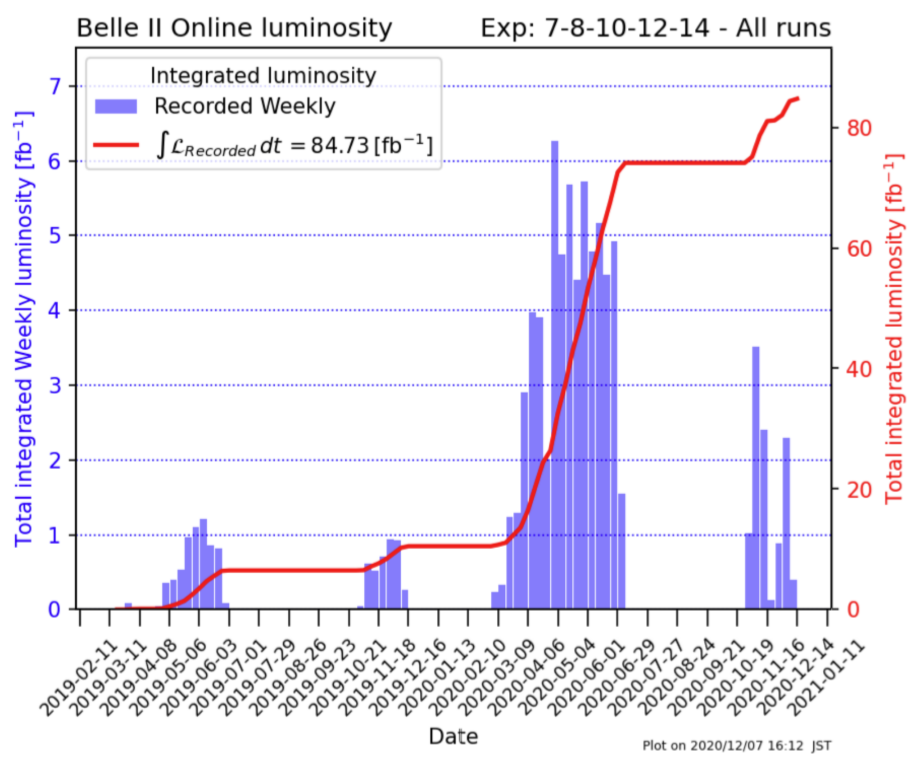
\includegraphics[width=0.6\linewidth]{b2lumi}
	\caption{Belle II online luminosity from 2019 April to the end of 2020\cite{b2onlinelumi}.}
	\label{fig:b2lumi} 
\end{figure}
% 2021.02.01 ends